%!TEX root = ../dissertation.tex

\chapter{Background}
\label{chapter:background}

%\section{The Internet of Things}

\section{Low Power Wide Area Networks}

%The number of \gls{IoT} devices is expected to grow significantly in the years to come. The year 2017 will be remembered as the year in which the number of connected devices surpassed the world population \footnote{https://www.statista.com/statistics/764026/number-of-iot-devices-in-use-worldwide/}.
In many applications, such as smart cities, environmental monitoring and smart agriculture, \gls{IoT} devices are densely deployed and powered by traditional AA batteries. For this reason, they must be able to operate under strict power constraints using simple and cheap hardware components. Transmitting data over a wireless medium is a very costly operation in terms of power, due to many unpredictable environmental factors such as heat, humidity, wind and buildings and due to the inherent complexity of traditional wireless technologies.
Protocols like \gls{BLE} and ZigBee try to address the power limitation problem for short-range communications, but for a vast number of \gls{IoT} applications, where a high number of devices are deployed over large areas (e.g. a city), short range solutions are suboptimal and expensive due to the complex and dense network infrastructure that needs to be installed and maintained. Existing technologies, such as cellular networks, cover large areas, but are not power efficient. Moreover 2G, 3G and LTE are typically available in urban areas, but not always in suburban or rural areas. To address the aforementioned problems, a new range of protocols and technologies are being developed with the explicit purpose of enabling the operation of \glspl{LPWAN}. As the name suggests, \glspl{LPWAN} have the primary objective of providing low-power and low-cost connectivity over large geographical areas. The applications are multiple and diverse: smart cities, smart grids, smart metering, logistics, industrial monitoring, smart agriculture, etc.
Recently, all the principal \glspl{SDO} such as the \gls{IETF}, the \gls{IEEE}, the \gls{3GPP} and the \gls{ETSI} are intensifying their efforts in the standardization of \gls{LPWAN} protocols. Moreover, numerous consortiums and alliances works to promote specific \gls{LPWAN} technologies. Examples of such alliances are the LoRa Alliance promoting the LoRaWAN protocol, the Dash7 Alliance promoting the Dash7 Alliance protocol and the Wightless-SIG promoting the Weightless protocol. Even if the existing \gls{LPWAN} protocols and solutions are extremely diverse and address different niches in the same application segment, most of them use similar solutions to solve the same range of problems. The most relevant features are listed below:

\begin{itemize}
\item \textbf{Use of sub-GHz bands:} the vast majority of \gls{LPWAN} protocols take advantage of the good properties of sub-GHz bands in terms of attenuation, multipath fading and obstacle penetration. Moreover, sub-GHz bands are currently less congested than other available bands, such as the overly used 2.4 GHz band. Most \gls{LPWAN} technologies (e.g. LoRa and Sigfox) use unlicensed \gls{ISM} bands. Cellular operators are instead trying to exploit already owned licensed frequency bands. The use of unlicensed \gls{ISM} bands reduces the operational costs of running the network, but most of the available bands are subject to limitations imposed by the legislative authorities of each country. As an example, the 868.0-868.6 MHz band, the one used by LoRa, is subject in Europe to a 1\% duty cycle limitation \cite{ref:bg-regulations}, which means that, in a day, a single device can transmit for at most 14.4 minutes.

\item \textbf{Use of \gls{NB} or \gls{SS} modulations:} \gls{NB} modulations have the advantage of reducing the adverse effects of noise on the transmitted signals. Using these techniques, receivers can successfully recover severely attenuated signals and achieve a sensitivity level of -130 dBm and below. As an example, the LoRa Semtech SX1276 chip achieves a sensitivity level of -148 dBm \cite{ref:bg-sx1276}. On the other side, the small bandwidth only allows low data rates in the order of few kbps or even a few hundred of bps if an \gls{UNB} modulation is used. In this last case the bandwidth can be as low as 100 Hz. Some protocols, such as LoRa, use variations of \gls{SS} techniques to spread the narrowband signal over a wider bandwidth. The resulting signal has noise-like characteristics that makes it more resistant to jamming and eavesdropping and more resilient to interference. To overcome the less efficient use of bandwidth, \gls{SS} is typically used in conjunction with orthogonal codes. This allows multiple overlapping signals that are spread using different codes to be successfully recovered at the receiver.

\item \textbf{Low power operation:} in a \gls{LPWAN}, end devices are typically battery-powered and might need to operate using the same battery for many years. To reduce power consumption, \gls{LPWAN} networks are organized in a simple and efficient star topology or a star-of-stars topology, where all the devices are directly connect to one or multiple gateways or base stations. Multi-hop protocols are typically not used since some network nodes, called hot-spots, might experience more traffic than the others. Moreover, hot-spots have to listen periodically for new messages coming from the other nodes thus reducing their overall battery lifetime. Duty-cycling the devices, i.e. alternating ON-OFF communication periods, is another frequently used technique to reduce the power consumption.
For example, an uplink transmission can start only when new data is ready and a downlink reception can start only at a predefined scheduled time, usually following an uplink transmission. Simple random access ALOHA-like MAC protocols, requiring simple and cheap hardware and no synchronization, are typically used. Finally, to save on computational power, some complex operations, like detecting duplicated packets, are offloaded to the backend side of the network.

\item \textbf{Low cost deployment:} installing, maintaining and operating an \gls{LPWAN} network must be as cheap as possible. The price of \glspl{LPWAN} chips is usually in the order of a few dollars. This can be achieved by resorting to simple and sometimes inaccurate hardware components. The network backbone usually requires only few base stations to cover areas of tens of kilometres, thus additionally reducing the deployment cost of the network. Finally, most \gls{LPWAN} solutions use unlicensed \gls{ISM} bands thus avoiding wasting money for the acquisition of licenses.

\item \textbf{Scalability:} support of a large number of devices is usually achieved by diversifying as much as possible in time, space and channels. Since devices use simple hardware, this diversification is usually implemented in the backend by using multi-channel multi-antenna base stations to parallelize the reception of signals. Some protocols also implement mechanisms to dynamically adapt the data rate and to select the best channel, but given the strong link asymmetry of most \gls{LPWAN} solutions, this mechanism, highly reliant on downlink information transmitted by the base station, is typically quite limited.

\end{itemize}


\section{LoRaWAN} \label{sec:lorawan}

The LoRaWAN standard \cite{ref:bg-lorawan-spec}, promoted by the LoRa Alliance, defines the MAC layer and the network architecture of an \gls{LPWAN} network that uses the proprietary LoRa modulation as a physical layer technology. The complete LoRaWAN stack is shown in Figure \ref{fig:lorawan-stack}. An overview of the main LoRaWAN physical and MAC layer characteristics and features is given in the following sections.

\begin{figure}[h]
    \centering
    \includegraphics[width=1\textwidth]{images/lorawan-stack.pdf}
    \caption{LoRaWAN stack}
    \label{fig:lorawan-stack}
\end{figure}

\subsection{LoRaWAN Physical Layer}

LoRa is a proprietary modulation technique based on \gls{CSS} originally developed by Cycleo and then acquired by Semtech in 2012. As many other \gls{LPWAN} technologies, LoRa uses unlicensed sub-GHz bands (868 MHz in Europe, 915 MHz in North America, 433 MHz in Asia), therefore taking advantage of the good propagation properties of the spectrum. Since the LoRa modulation is proprietary, no official comprehensive description of the modulation exists as of today, but some attempts to reverse engineer the protocol have been made. The description of the LoRa physical layer given in the present work is partially based on the little information given in the official LoRaWAN standard \cite{ref:bg-lorawan-spec} and on Semtech technical documents, such as \cite{ref:bg-semtech-lora}. More in depth details are taken from the reverse engineering efforts undertaken by Knight et al. \cite{ref:bg-reversing-lora1} \cite{ref:bg-reversing-lora2}.

\subsubsection{LoRa Modulation}

\begin{figure}[h]
    \centering
    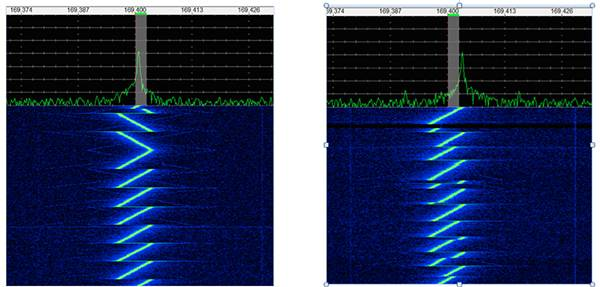
\includegraphics[width=1\textwidth]{images/lora-chirps.jpg}
    \caption{Visualisation of LoRa chirps (source: LinkLabs)}
    \label{fig:lora-chirps}
\end{figure}

The LoRa modulation is a variation of the \gls{CSS} modulation technique, which is in turn a subcategory of \gls{DSSS}. In \gls{DSSS} data is spread over a wider bandwidth by multiplying the transmitted symbol by a \gls{PN} sequence called chip sequence. The \gls{PN} sequence is generated with a frequency higher than the symbol generation frequency. The result is a signal with a very low \gls{SNR} that makes it practically unrecognisable from background noise and very resilient to other \gls{RF} noise sources. The \gls{PN} sequence, known also by the receiver, is used to de-spread the signal and recover the original data. These properties make \gls{DSSS} an ideal solution for \glspl{LPWAN}. Unfortunately, \gls{DSSS} requires a highly accurate and expensive clock source to synchronize the \gls{PN} sequence at the transmitter and at the receiver. This makes traditional \gls{DSSS} not particularly suited for low-cost end devices such as the ones deployed in a \gls{LPWAN}.
\gls{CSS} is a variation of \gls{DSSS} initially used for radar systems and for a long time ignored in communication systems, but recently revalued due to its robustness to a wide range of channel degradation mechanisms such as multipath fading, signal fading, Doppler shift and jamming interferers.
In \gls{CSS}, the chip sequences are substituted by chirps, i.e. signals of continuously increasing or decreasing frequency inside a defined frequency range. An increasing frequency chirp is called up-chirp, while a decreasing frequency chirp is called down-chirp. To simplify transmitter and receiver's hardware, up-chirps and down-chirps are typically linear in frequency as is the case for LoRa.
In LoRa, a symbol is first chipped at a higher frequency that depends on the \gls{SF} and then modulated into a chirp. The chirp is characterized by the \gls{SF}, a minimum frequency $f_{min}$ and a maximum frequency $f_{max}$. An initial frequency $f_0$ is assigned to the symbol. The chirp sweeps the frequencies from $f_0$ to $f_{max}$, wrapping around from $f_{max}$ to $f_0$ when hitting the end of the available bandwidth $B = f_{max} - f_{min}$. A visualization of LoRa \gls{CSS} can be seen in Figure \ref{fig:lora-chirps}. The period of the chirp is determined by Equation \ref{eq:chirp_period}. The modulation data rate can then be computed as shown in Equation \ref{eq:lora_dr}.

\begin{equation}
\label{eq:chirp_period}
T_C = \frac{2^{SF}}{B} secs
\end{equation}

\begin{equation}
\label{eq:lora_dr}
R_b = SF*\frac{1}{T_C} bits/s
\end{equation}

From equations \ref{eq:chirp_period} and \ref{eq:lora_dr}, it is possible to observe that a bigger \gls{SF} corresponds to a longer chirp period and consequently a lower data rate. On the other side a higher \gls{SF} makes the signal more resilient to noise and other \gls{RF} interferers, thus allowing for a lower receiver sensitivity and therefore the possibility of successfully recovering the signal from higher distances. This robustness is counterbalanced by a higher probability of collision, since the signal takes more time to be transmitted. In LoRa the \gls{SF} can vary between 7 and 12. If the coding rate is not considered, the typical LoRa data rates can be easily computed and are presented in Table \ref{tab:lora_dr}.

\begin{table}[]
\centering

\begin{tabular}{|c|c|c|}
\hline
\textbf{SF} & \textbf{Bandwidth} & \textbf{Bitrate} \\ \hline
 12 & 125 kHz & 366 bps  \\ \hline
 11 & 125 kHz & 671 bps \\ \hline
 10 & 125 kHz & 1220 bps \\ \hline
  9 & 125 kHz & 2197 bps \\ \hline
  8 & 125 kHz & 3906 bps \\ \hline 
  7 & 125 kHz & 6835 bps \\ \hline 
\end{tabular}
\caption{LoRa Data Rates}
\label{tab:lora_dr}

\end{table}

\subsubsection{LoRa Physical Layer Packet}

The LoRa phisical layer packet is composed of three fields:

\begin{itemize}

\item \textbf{Preamble:} used for the synchronization between the receiver and the transmitter. It's composed of a variable sequence of up-chirps having the same duration;

\item \textbf{\gls{SFD}:} indicates the beginning of a frame. It's composed by 2 down-chirps;

\item \textbf{Header and Data:} up-chirps of varying length. The data is extracted from the instantaneous frequency transitions of the chirps.

\end{itemize}

Some additional techniques are used to increase the robustness of the LoRa modulation:

\begin{itemize}

\item \textbf{Gray Indexing:} before being transmitted, the symbols are Gray indexed. Gray indexing is a way of encoding digits such that two consecutive digits have a change only in one bit position. This allows for more error tolerance. In the actual implementation, the symbols are read as gray-coded and de-grayed before transmission. Therefore the decoder needs to gray-code the symbols to recover the original symbols;

\item \textbf{Data whitening:} this process induces randomness in the sequence of bits in order to reduce long sequences of repeating bits. This allows a better clock recovery by the receiver. The whitening is done by XORing the symbols with a pseudorandom sequence that is known by both the transmitter and the receiver;
    
\item \textbf{Interleaving:} the initial ordered sequence of bits is scrambled using a scrambling sequence. The receiver uses the inverse operation to reconstruct the original bit sequence. This technique is used in conjunction with \gls{FEC} to spread multiple consecutive errors over the whole frame. LoRa uses a variation of a diagonal interleaver;

\item \textbf{\gls{FEC}:} enables bits damaged during the transmission to be recovered at the receiver by introducing some redundancy in the transmitted data. LoRa implements a Hamming \gls{FEC} that substitutes a 4-bit word with a codeword with length in the range [5-8] bits. A longer codeword provides additional protection at the cost of additional bits. When an Hamming (5,4) or (6,4) is used, only error detection is available. A Hamming (7,4) can correct a single bit error, while a Hamming (8,4) can correct a two bit error.

\end{itemize}

To improve reliability, code diversity is also exploited. Different spreading factors use semi-orthogonal codes, thus enabling the recovery of two signals overlapping in time and frequency if they have different \glspl{SF}. This feature allows the network to achieve a higher overall throughput, thanks to the fact that colliding packets with different \glspl{SF} can still be correctly demodulated.

%\subsection{LoRaWAN Architecture and MAC Layer}
%
%The architecture and the MAC layer of LoRaWAN are defined as an open standard that is currently in its 1.1 version. In this section an overview of the main features of 

\subsection{Architecture and Topology}

\begin{figure}[h]
    \centering
    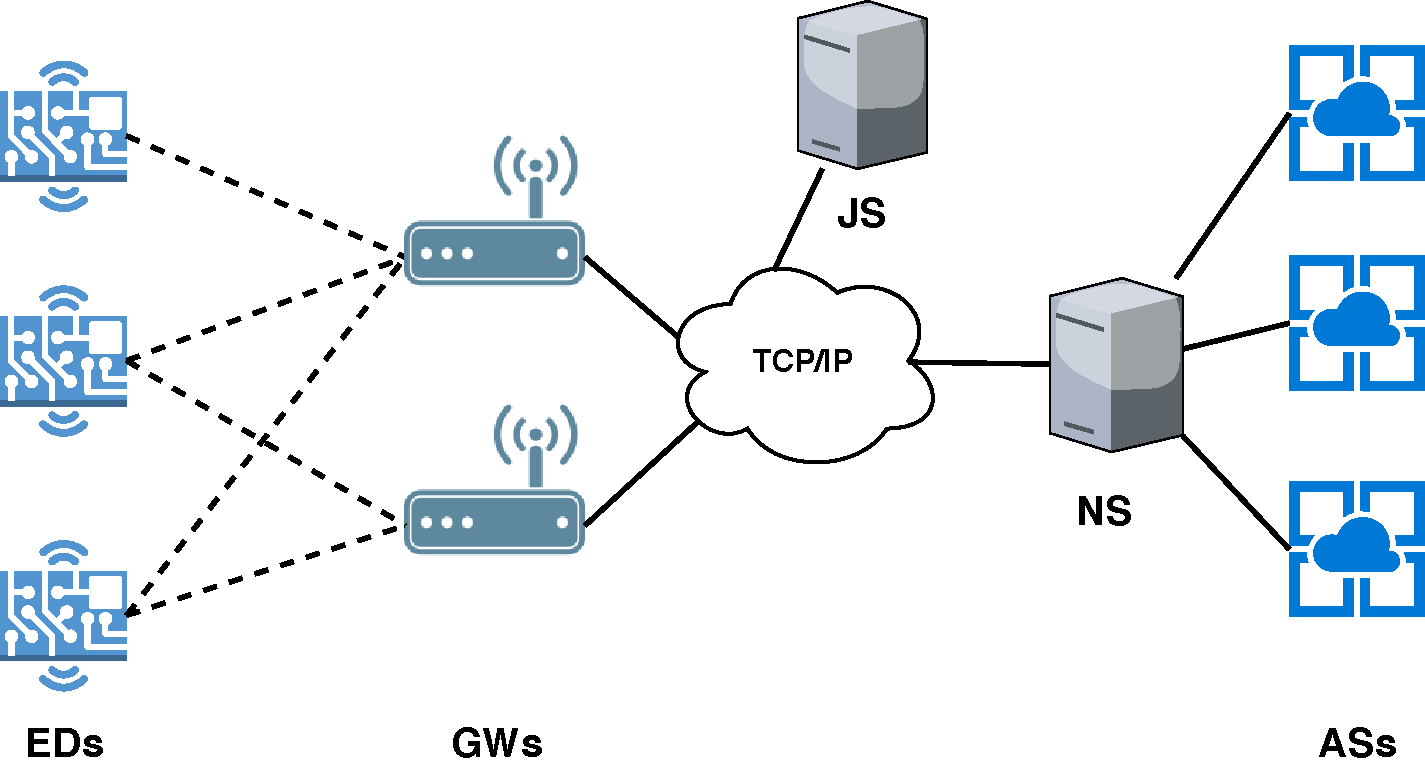
\includegraphics[width=0.95\textwidth]{images/lora-topology.pdf}
    \caption{Topology of a LoRaWAN network}
    \label{fig:lorawan-architecture}
\end{figure}

The overall architecture of LoRaWAN is shown in Figure \ref{fig:lorawan-architecture}.
LoRaWAN implements a star-of-stars topology interconnecting five different network elements:

\begin{itemize}
	\item \textbf{\glspl{ED}:} they are typically low-powered devices with sensing capabilities. \glspl{ED} transmit or receive data using the LoRa radio channel. They can establish communication only with LoRa gateways.
Once an \gls{ED} is registered in the network, uplink messages can be received by multiple gateways at once;

	\item \textbf{\glspl{GW}:} one or multiple gateways are responsible for collecting and aggregating the data coming from the \glspl{ED}. Gateways are responsible for demodulating the LoRa uplink transmissions and relaying the uplink messages to a network server using a traditional IP-based backhaul network. Upon request, \glspl{GW} can also send downlink messages to \glspl{ED};
	
	\item \textbf{\gls{NS}:} collects the packets coming from the \glspl{GW} and routes them to the appropriate \gls{AS}. The \gls{NS} is also responsible for sending and receiving MAC commands and discard duplicated packets;
	
    \item \textbf{Application Servers (ASs)}: implement the application specific logic. An \gls{AS} aggregates, analyses and/or stores data and present it to the end users in a meaningful way. End users only interact with the services offered by an \gls{AS};
    
    \item \textbf{\gls{JS}:} manages \glspl{ED} activation. It derives and stores the keys used by the network for encrypting the communications.
        
\end{itemize}

\subsection{\glspl{ED} Operation Modes}

LoRaWAN defines three classes of \glspl{ED} with different characteristics and functionalities:

\begin{itemize}
 \item \textbf{Class A \glspl{ED}:} class A is the default operation mode of a LoRaWAN device. Class A \glspl{ED} open two short downlink receive windows immediately after an uplink transmission, therefore making this mode of operation best suited for \glspl{ED} that need a feedback from the network only after a successful transmission. The first receive window (RX1) is opened immediately after the uplink transmission. During RX1, the downlink frequency and data rate are set according to the same set of parameters used in uplink. In the second receive window (RX2), the downlink frequency and data rate are fixed and can be configured using specific MAC commands. Both RX1 and RX2 must stay open at least for the time needed for a \gls{GW} to detect the downlink preamble and are only closed when the eventual downlink transmission is completed. Thanks to the short and limited downlink periods, Class A \glspl{ED} are the most power-efficient devices in a LoRaWAN network;
 
\item \textbf{Class B \glspl{ED}:} these devices retains all the functionalities of class A \glspl{ED} and furthermore, they can open additional receive windows at specific time instants agreed with the \glspl{GW}. \glspl{GW} must periodically send a beacon that specifies the exact time at which the additional receive windows must be opened. This feature allows for a more flexible use of the downlink channel, therefore representing a good compromise in terms of power consumption and chances of sending downlink messages;

\item \textbf{Class C \glspl{ED}:} \glspl{ED} operating in this mode keep the receiving windows continuously open, except when the ED is transmitting a message in uplink. Class C operation mode is the least power-efficient class and should only be used for \glspl{ED} with relaxed power constraints that benefit from low latency downlink messages.

\end{itemize}

All the \glspl{ED} must implement Class A operation mode and may optionally implement one or all of the other available classes. An \gls{ED} can switch to Class B or Class C operation modes by using specific MAC commands only after having successfully joined the LoRaWAN network. 

\subsection{MAC Frames and Commands}

\begin{figure}[h]
    \centering
    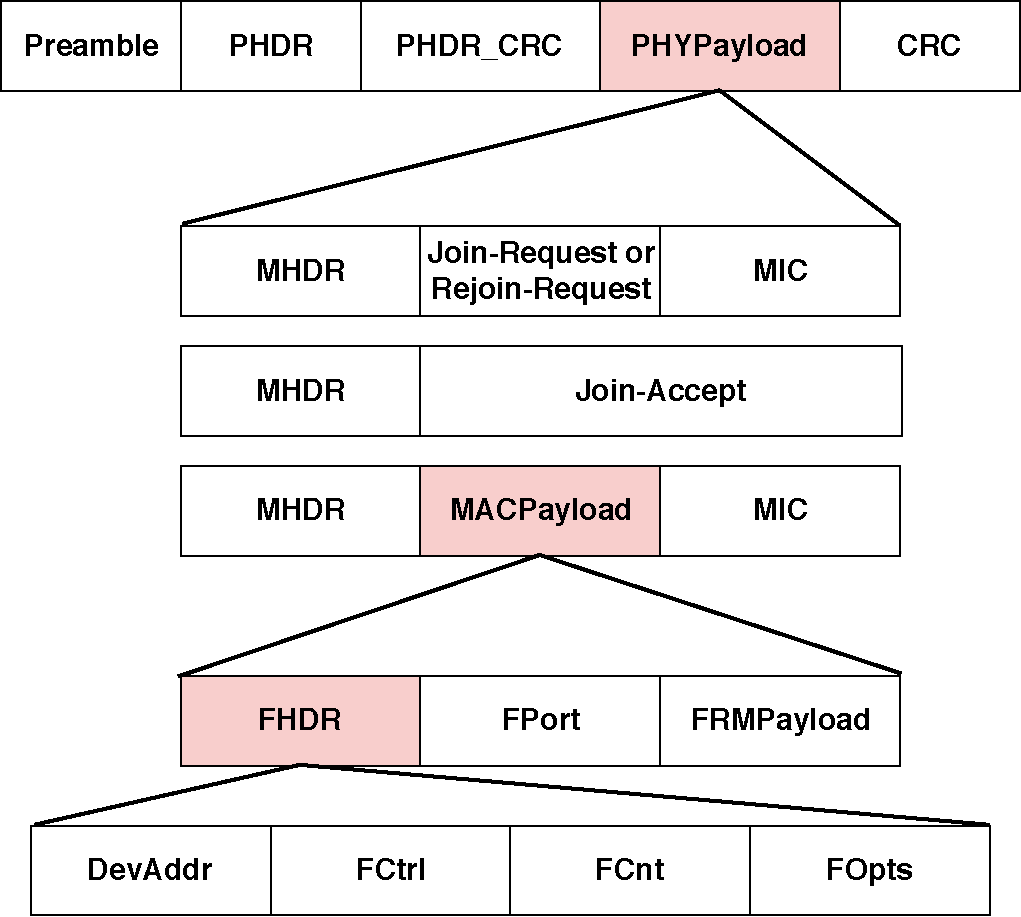
\includegraphics[width=0.9\textwidth]{images/mac-commands.pdf}
    \caption{MAC frames structure}
    \label{fig:lorawan-mac}
\end{figure}

The structure of LoRaWAN MAC frames is shown in Figure \ref{fig:lorawan-mac}.
MAC frames are encapsulated in the physical layer packet payload and are formed by a \gls{MHDR}, a MAC payload (MACPayload) and a \gls{MIC}, that is used to verify the integrity of the PHY payload. 
The \gls{MHDR} contains, among other fields, a 3-bit MType field that specifies the message type. The available types are listed in Table \ref{tab:mtypes}.

\begin{table}[]
\centering

\begin{tabular}{|c|c|}
\hline
\textbf{MType} & \textbf{Description}\\ \hline
 000 & Join-Request  \\ \hline
 001 & Join-Accept \\ \hline
 010 & Unconfirmed Data Up  \\ \hline
 011 & Unconfirmed Data Down  \\ \hline
 100 & Confirmed Data Up \\ \hline 
 101 & Confirmed Data Down \\ \hline
 110 & Rejoin-Request \\ \hline  
 111 & Proprietary \\ \hline 
\end{tabular}
\caption{MAC message types (MTypes)}
\label{tab:mtypes}

\end{table}

Data messages are used for transmitting MAC commands and/or application data. A distinction is made between data messages that require an acknowledgement from the receiving device (an \gls{ED} or a \gls{GW}) and data messages that do not require an explicit acknowledgement. Join-request, Join-Accept and Rejoin-request messages are used for \gls{OTA} activation as described in section \ref{sec:activation}.  
The MACPayload field is additionally divided in \gls{FHDR}, \gls{FPort} and Frame Payload (FRMPayload). The \gls{FHDR} contains a 4-byte Device Address (DevAddr), a 1-byte Frame Control (FCtrl) to request the \gls{ADR} or an acknowledgement, a 2-byte Frame Counter (FCnt) and an optional Frame Options (FOpts) field containing up to 15 bytes of MAC commands. The mandatory 1-byte \gls{FPort} field is used to specify the port used by the application. This field is used by the \gls{NS} to route the message to the correct application in the \gls{AS}.
Other than data, LoRaWAN MAC frames can carry one or more MAC commands.  
MAC commands are simple commands exchanged exclusively between the \gls{NS} and the \glspl{ED}. MAC commands can be piggybacked to a data message using the FOpts field or they can be carried in the FRMPayload by specifying a FPort value of 0. Each command is defined by a 1-byte \gls{CID} followed by zero or more command specific octets.
MAC commands can be used to:

\begin{itemize}
 
    \item Check the line connectivity;
    \item Limit the duty cycle of an \gls{ED};
    \item Set the receive parameters of the second receive window;
    \item Request status info to \glspl{ED};
    \item Set the delay between a transmission and the opening of the first receive window;
    \item Change \gls{ADR} parameters;
    \item Request current time and date to the network.

\end{itemize}

\subsection{Adaptive Data Rate}

% Revise. Probably not specific enough

LoRaWAN specifies an \gls{ADR} mechanism that is used to optimize the data rate, transmission power and spectrum usage of \glspl{ED} according to the quality of the link as measured by different metrics. When \gls{ADR} is active, the \gls{SF} of the modulation is adjusted in order to match the quality of the channel: it is increased when the \gls{SNR} is low in order to increase the receiver sensitivity and decreased when the \gls{SNR} is well above the threshold in order to minimize the power consumption and the time-on-air of the messages. An \gls{ADR} request is always started by an \gls{ED} by setting the \gls{ADR} bit in the FCtrl field. This bit signals to the \gls{NS} that the node is willing to accept \gls{ADR} parameters variations based on the observations collected by the \gls{NS}. The \gls{ADR} should only be used by static nodes or by "smart" mobile nodes that are able to detect when they are parked for an extended period of time. \\
The \gls{ADR} algorithm runs asynchronously in both the \gls{ED} and the \gls{NS}. The algorithm running on the \gls{ED} is specified by the LoRa Alliance and consists in a progressive increment of the \gls{SF} after a predefined number of downlink frames is not received. According to this algorithm, the \gls{SF} can only be increased. To overcome this limitation, an \gls{ADR} algorithm can be set up in the \gls{NS}. It's worth noting that the specification doesn't specify an algorithm to be used for \gls{ADR} in the \gls{NS}, thus leaving the implementation details to the manufacturer of the network equipment or the network operator. As an example, Semtech suggests a simple \gls{ADR} algorithm: when \gls{ADR} is requested, the \gls{NS} starts collecting the uplink frames sent by the \gls{ED} and uses the 20 most recent ones to compute

\begin{equation}
	SNR_{margin} = \max_{20 \ frames} (SNR) - SNR (DR) - margin\_db
\end{equation}

where $SNR (DR)$ is the minimum required SNR necessary to correctly demodulate the signal for the incoming \gls{SF} and $margin\_db$ is a device specific margin that is typically set to 10 dB. $SNR_{margin}$ is used to compute the parameter

\begin{equation}
	N_{step} = \left \lceil{SNR_{margin}/3} \right \rceil
\end{equation}

which can be positive or negative. If $N_{step}$ is positive and the \gls{SF} is bigger than the minimum allowed, the \gls{SF} is decremented by $N_{step}$. If instead the \gls{SF} is already at its minimum, the transmission power is decremented by $3 \times N_{step}$ dB. Finally, if $N_{step}$ is negative, the transmission power is increased by $3 \times N_{step}$ dB.


 
%\begin{algorithm}[H]
% \KwData{this text}
% \KwResult{how to write algorithm with \LaTeX2e }
% initialization\;
% \While{not at end of this document}{
%  read current\;
%  \eIf{understand}{
%   go to next section\;
%   current section becomes this one\;
%   }{
%   go back to the beginning of current section\;
%  }
% }
% \caption{How to write algorithms}
% \label{alg:adr}
%\end{algorithm}


%http://flora.aalto.fi/download/slabicki2018adaptive.pdf extend with info in here

\subsection{Activation of \glspl{ED}}

A LoRaWAN network implementation is by default protected by some security mechanisms that ensure data integrity and confidentiality and prevent replay attacks. These three requirements are guaranteed respectively by \glspl{MIC}, 128 bits \gls{AES} encryption and nonces. All security features require the presence of a set of session keys, that must be derived during the \gls{ED} mandatory join procedure.
Each \gls{ED} must join the network using either \gls{OTA} activation or \gls{ABP}. The only difference between the two procedures is in the way in which the session keys are derived: in \gls{OTA} activation, keys are generated on-demand, while in \gls{ABP} keys are manually loaded. Only the most interesting \gls{OTA} activation is discussed in this section. \\

\subsubsection{OTA Activation} \label{sec:activation}

Before starting the join procedure, each \gls{ED} is provided with four pieces of information that must be stored securely in the device:

\begin{itemize}
	\item \textbf{Join EUI:} a 64 bit global identifier of the \gls{JS} responsible for the join procedure;
	\item \textbf{Device EUI (DevEUI):} a 64 bit global identifier of the \gls{ED}. The DevEUI is typically written also on a label on the back of the \gls{ED};
	\item \textbf{Network Key (NwkKey):} an AES-128 root key, assigned when the \gls{ED} is manufactured, used to derive the Forwarding Network Session Integrity Key (FNwkSIntKey), the Serving Network Session Integrity Key (SNwkSIntKey) and the Network Session Encryption Key (NwkSEncKey);
	\item \textbf{Application Key (AppKey):} an AES-128 root key, assigned when the \gls{ED} is manufactured, used to derive the Application Session Key (AppSKey).
\end{itemize}

The join procedure is always started by an \gls{ED} by sending a Join-Request message to the \gls{JS} containing the Join EUI, the DevEUI and a Device Nonce (DevNonce). The DevNonce is used to avoid the occurrence of replay attacks. The \gls{ED} must store the last used DevNonce value and increment it at each subsequent Join-Request. The last value of the nonce is also permanently stored in the \gls{NS} and every time a message is received, the DevNonce is compared with the stored value. If the received nonce is lower than the value stored in the \gls{NS}, the message is discarded. If the \gls{JS} accept the \gls{ED} registration, a Join-Accept message is returned in downlink. The message contains the join nonce, the Network id (NetID), the 32-bit Device Address (DevAddr) and a set of network configuration parameters. The join nonce is also in this case a progressive number, but it is used to derive the session keys. After the completion of the join procedure, the following session keys are established:

\begin{itemize}

\item \textbf{FNwkSIntKey:} used by the \gls{ED} to compute the \gls{MIC} of all uplink messages;
\item \textbf{SNwkSIntKey:} used by the \gls{ED} to verify the \gls{MIC} of all downlink messages;
\item \textbf{NwkSEncKey:} used by the \gls{ED} and the \gls{NS} to encrypt/decrypt uplink and downlink MAC commands;
\item \textbf{AppSKey:} used by the \gls{ED} and the \gls{AS} to encrypt end-to-end the payload field of application-specific data messages. It's worth noting that even if confidentiality is guaranteed end-to-end, the integrity of messages is only guaranteed hop-by-hop, thus potentially allowing a malicious \gls{NS} to tamper with the data;

\end{itemize}

% --------------------  REVISED TILL HERE -------------

\section{The IEEE 802.11 Protocol}

% Description of WiFi protocol

\gls{IEEE} 802.11, best known as WiFi, is a widely used MAC and Physical (PHY) layer protocol suite for establishing wireless \glspl{LAN} operating in the license-free 900 MHz, 2.4 GHz, 5.7 GHz and 60 GHz \gls{ISM} bands. The first version of the standard was published in 1997 by the \gls{IEEE}. Since then, many revisions of the protocol have been issued, most of them targeting mainly the PHY layer with the explicit purpose of increasing the maximum achievable throughput. The most relevant PHY amendments (IEEE 802.11a/b/g/n/ac) are discussed in this section. Also the MAC layer received some upgrades over the years in order to improve specifics aspects, like QoS (IEEE 802.11e), security (IEEE 802.11i) and throughput (IEEE 802.11n). In this section, the original MAC specification and the most relevant modifications introduced with IEEE 802.11n are discussed.

\subsection{IEEE 802.11 Architecture}

\begin{figure}[h]
    \centering
    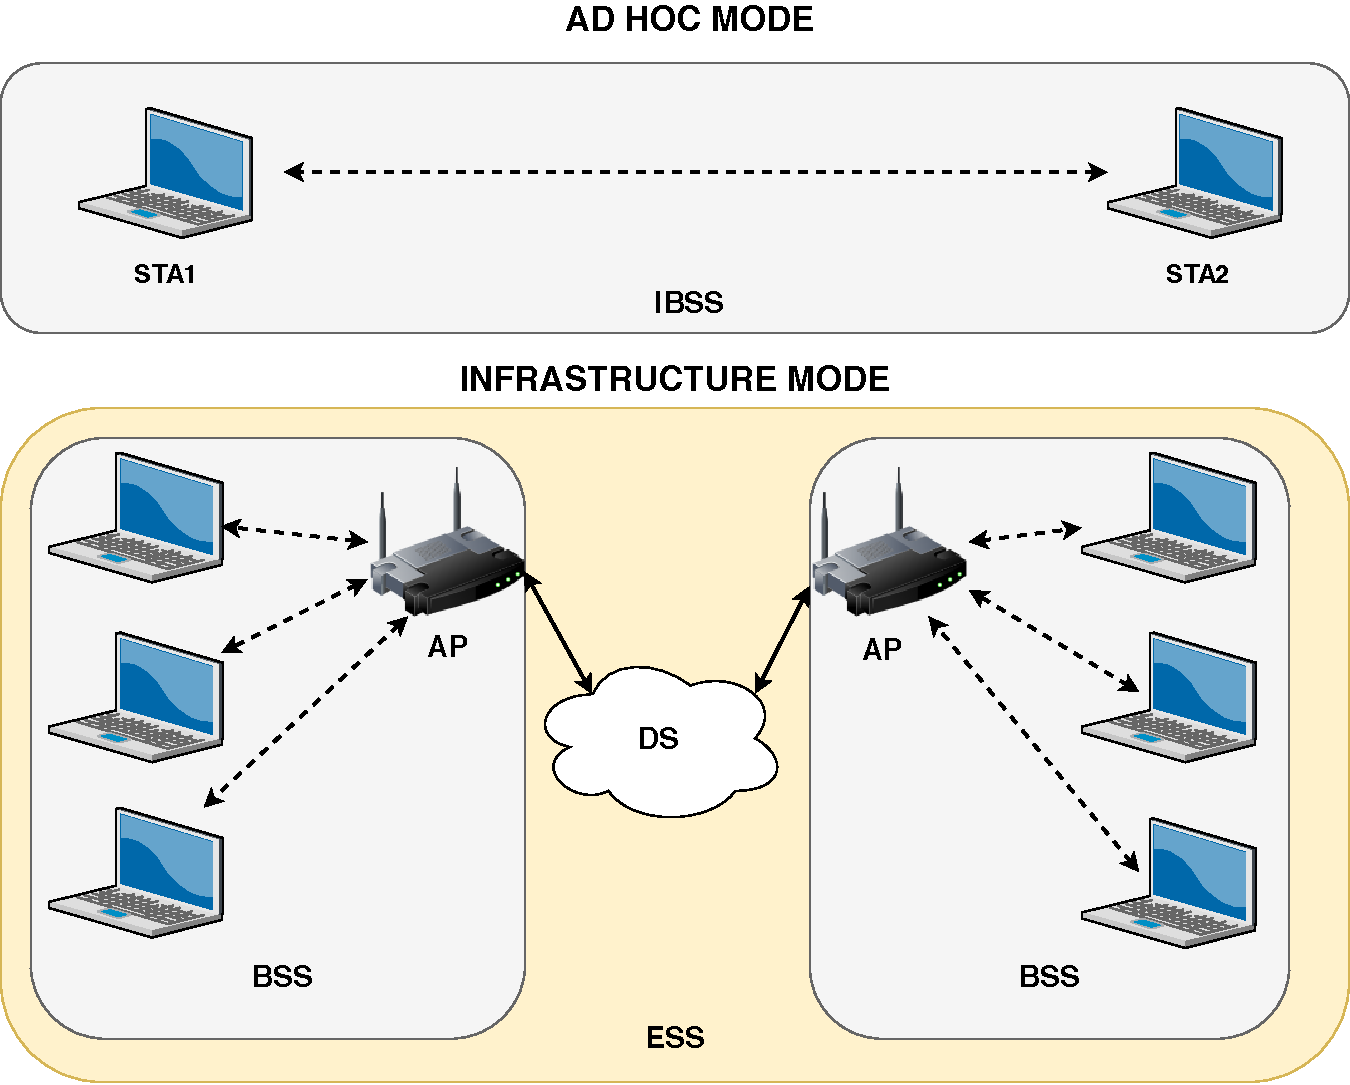
\includegraphics[width=1\textwidth]{images/wifi-architecture.pdf}
    \caption{Architecture of an IEEE 802.11 network}
    \label{fig:wifi-architecture}
\end{figure}

An IEEE 802.11 network can operate in one of two modes: ad-hoc mode or infrastructure mode. In ad-hoc mode each \gls{STA} can only establish a direct communication with other \glspl{STA} in their wireless coverage area, forming in this way an \gls{IBSS}. In infrastructure mode, \glspl{STA} connect exclusively to a special distribution \gls{STA}, called \gls{AP}, that must take care of coordinating and bridging the traffic among the connected \glspl{STA}. An \gls{AP} and its associated \glspl{STA} form what is called an infrastructure \gls{BSS}, characterized by a unique \gls{BSSID} (corresponding to the MAC of the \gls{AP}) and a \gls{SSID}. To extend the coverage of the network, multiple infrastructure \gls{BSS} can be interconnected through their \glspl{AP} by a \gls{DS}. The set of infrastructure \gls{BSS} having the same \gls{SSID} and interconnected by a \gls{DS}, form an \gls{ESS}.
Both ad hoc mode and infrastructure mode architectures are depicted in Figure \ref{fig:wifi-architecture}.

\subsection{IEEE 802.11 MAC Layer}

IEEE 802.11 MAC layer is responsible for reliable data delivery, access control and security. The IEEE 802.11 MAC protocol, known as \gls{DFWMAC}, provides both a mandatory decentralized, contention-based access protocol called \gls{DCF} and an optional centralized, contention-free protocol called \gls{PCF}. \\\\
The \gls{DCF} uses \gls{CSMA} to access the medium. According to this technique, each station listens to the medium and starts the transmission only if no other station is transmitting. If the medium is busy, the transmission is deferred to a later time after a backoff time chosen at random. \gls{CSMA} with \gls{CD} is typically used in wired media and it relies on the capability of all stations to receive a feedback in case a collision occurs. This assumption is not valid in wireless media, since not all stations are in the communication range of all the other stations participating in the network. Therefore a collision might occur at the receiver and go undetected at the transmitter. This issue is known as the hidden terminal problem. To overcome this complication, the \gls{DCF} uses \gls{CSMA} with \gls{CA}. As specified by this protocol, the transmitting station senses the medium for a fixed amount of time (\gls{DIFS}) and if at the end of the period the medium is still free, the frame is sent, otherwise a back-off time is uniformly chosen in the interval $[0, CW]$ and progressively decremented during the channel idle times. The value of $CW$ starts at $CW_{min}$ and it is doubled at every collision up to $CW_{max}$. When a data frame is successfully received, the receiving station, after a short fixed interval (\gls{SIFS}), replies with an acknowledgement frame (ACK). If the ACK is not received before the expiration of a timeout, a collision happened at the receiver and the sender needs to retransmit the frame. The medium access priority is determined by \glspl{IFS} of varying length, such that a larger \gls{IFS} implies a lower priority transmission. Since a \gls{SIFS} is smaller than a \gls{DIFS}, frames associated with \gls{SIFS}, like ACKs, have a higher probability of taking control of the channel. To reduce even more the chances of collisions, the \gls{DCF} implements an optional virtual carrier sense mechanism based on \gls{RTS} and \gls{CTS} frames. After \gls{DIFS}, a transmitter can send a \gls{RTS} frame with the indication of the reservation parameters. If the sender is allowed to transmit, the receiver replies with a \gls{CTS}. At this point, the exchange continues with the transmission of a data frame and the following ACK frame. Stations that are listening to the medium receives \gls{RTS} or \gls{CTS} frames containing the duration of the transmission and react by setting the \gls{NAV}, which is an indicator of how much a station should defer the access to the medium. In this way, even if a station is not able to hear the transmission of another station, it can determine that someone is transmitting simply by detecting an outgoing \gls{CTS} frame. \\\\
The \gls{PCF} relies on a centralized polling mechanism and it's therefore available only to networks working in infrastructure mode, where the \gls{AP} acts as polling coordinator. In order for \gls{PCF} and \gls{DCF} to coexist, time is divided in slots called \textit{superframes}. The first part of a superframe is reserved for contention-free access. During this time, the polling coordinator gains control of the medium by waiting for the duration of a \gls{PIFS} (which is shorter than a \gls{DIFS}) and then sending a beacon that specifies the maximum duration of the \gls{PCF} period. All the stations receiving the beacon set their \gls{NAV} according to the specified duration. Finally, the polling coordinator polls the stations in the polling list one by one. \\ \\
The correct operation of a IEEE 802.11 network depends on the periodic broadcast of beacon frames containing information about the \gls{BSS}, e.g. the timestamp, the beacon interval, the \gls{SSID}, the capabilities of the network, the \gls{DSSS} parameters and the \gls{PCF} parameters. Moreover beacons are necessary for synchronizing the stations in the \gls{BSS}. Beacons periodic broadcasting is typically performed by the \gls{AP}, but in a \gls{IBSS}, due to the lack of a central coordinator, such function is taken in turn by all the stations. Each station randomly sets a timer and a beacon is sent when the timer expires and no other beacon is received in the meanwhile. \\ \\
With IEEE 802.11n, some MAC enhancements have been introduced to achieve higher throughputs. The main introduction is the aggregation of multiple data packets coming from the transport layer in one single frame. This technique reduces the impact of the inter frame time and of the MAC overhead. Two aggregation methods are defined: \gls{A-MSDU} and \gls{A-MPDU}. An \gls{A-MSDU} aggregates multiple \glspl{MSDU}. Since a single MAC header is generated for each \gls{A-MSDU}, all the aggregated frames must have the same source and destination address. Conversely, an \gls{A-MPDU} can aggregate multiple \glspl{MPDU}, each one with its own MAC header and possibly different source and destination addresses, and eventually even multiple \glspl{A-MSDU}. This difference is particularly relevant in combination with another mechanism introduced by the protocol: block acknowledgements. According to this mechanism, upon reception of an \gls{A-MPDU}, the receiver responds with an ACK containing only the indication of the correctly received \glspl{MPDU}. Therefore only \glspl{MPDU} with errors need to be retransmitted.

%Something about MAC enhancements of 802.11n + maybe MAC frame structure

\subsection{IEEE 802.11 PHY Layer} \label{sec:wifi-phy}

The IEEE 802.11 PHY layer evolved rapidly after the first 1997 draft. The first version of the standard, never actually implemented, specifies a physical layer based on \gls{DSSS} and \gls{FHSS}, with a maximum bitrate of 2 Mbps. Since then, many amendments, improving the efficiency and the bitrate of the PHY layer have been issued. 
%Table \ref{table} summarizes some of the most important features of each amendment.

%Describe channel structure...
\begin{figure}[h]
    \centering
    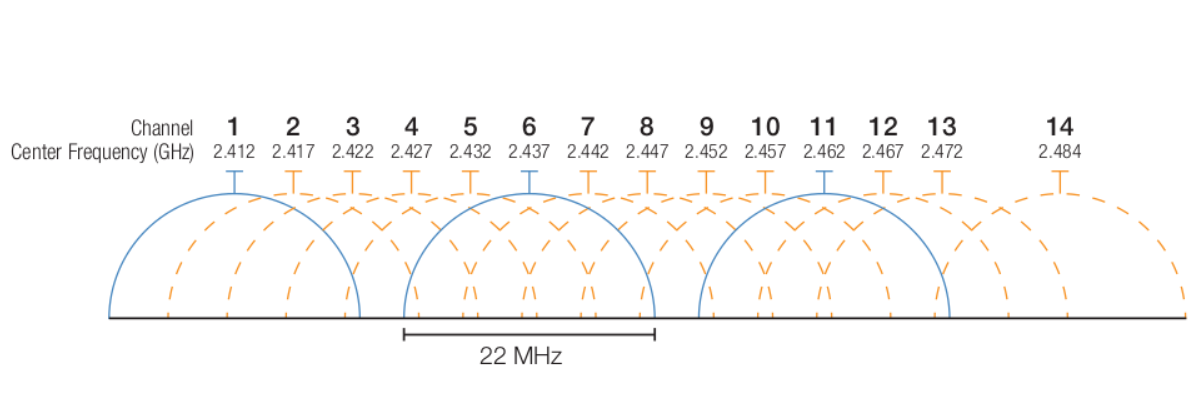
\includegraphics[width=1\textwidth]{images/wifi-channels-24.png}
    \caption{Channels in the 2.4 GHz band \cite{appinwififolder}}
    \label{fig:wifi-channels-24}
\end{figure}


\subsubsection{IEEE 802.11b}

IEEE 802.11b is the first revision that has been broadly implemented in consumer and enterprise devices. It shares with the original PHY implementation the use of the \gls{DSSS} modulation and of the 2.4 GHz band, but with the advantage of an increased maximum raw bitrate that reaches 11 Mbit/s. This huge bitrate increment was made possible by substituting the Barker's code used in \gls{DSSS} with the more efficient Complementary Code Keying, that allowed for more bits to be encoded in the spreading sequence. The most critical part of 802.11b is the use of the 2.4 GHz band, that is used by many electro-domestic devices. Moreover, as shown in Figure \ref{fig:wifi-channels-24}, depending on regional regulations, only three or four 20 MHz-wide non-overlapping channels are available in the 2.4 GHz band, thus increasing the chance of interference.

\subsubsection{IEEE 802.11a}

IEEE 802.11a has been released almost at the same time of IEEE 802.11b, but has never been widely adopted, due to the popularity of IEEE 802.11b and the high cost of producing hardware operating in the 5 GHz band. This revision substitutes the original \gls{DSSS} modulation with a more efficient \gls{OFDM} with 52 sub-carriers, that allows a maximum bitrate of 54 Mbit/s. The biggest advantage of IEEE 802.11a over IEEE 802.11b is the use of the 5 GHz band, which is far less congested than the 2.4 GHz band. Moreover, the presence of 24 non-overlapping channels guarantees a significant increase in capacity. The only disadvantage is the slightly reduced range due to the worse propagation characteristics of the signal at higher frequencies, but this is counterbalanced by the good properties of \gls{OFDM} in terms of attenuation of the effects of multipath fading.

\subsubsection{802.11g}

IEEE 802.11g has been issued in 2003 and immediately became very popular, thanks to the rapid increase in demand of higher throughput wireless networks. To maintain the compatibility with IEEE 802.11b, this new revision operates in the 2.4 GHz band and offers some additional mechanisms to ensure interoperability between the two protocols. This comes at the expense of the maximum achievable throughput in mixed 802.11b/g networks. IEEE 802.11g uses the same \gls{OFDM} modulation used by IEEE 802.11a, thus achieving a maximum bitrate of 54 Mbit/s. For backward compatibility, lower data rates with \gls{DSSS} and Complementary Code Keying are supported.

\subsubsection{802.11n}

IEEE 802.11n introduces enhancements to both the PHY and MAC layer that allow to reach a maximum bitrate of 600 Mbit/s. This is made possible by taking advantage of wider channels (40 MHz), shorter guard bands (400 ns) and especially multiple antennas (MIMO) that can differentiate up to four simultaneous spatial streams in the same channel. Beamforming is also supported. The standard can operate on both the 2.4 GHz and the 5 GHz bands, but protection mechanisms need to be established in the 2.4 GHz band to avoid interference with legacy devices. In fact, using a 40 MHz channel results in the occupation of 9 of the 14 available channels of the 2.4 GHz band. The standard support various combinations of modulation schemes (up to 64 QAM) and coding rates (up to 5/6), that allow to adapt the data rates to the condition of the channel and of the environment.

\subsubsection{802.11ac}

IEEE 802.11ac builds on the features of IEEE 802.11n and introduces enhancements with the explicit purpose of supporting very high throughput applications, such as multimedia applications. The standard now supports the bonding of four channels (80 MHz) or eight channels (160 MHz), a denser modulation (256 QAM) and even more MIMO streams (up to 8 simultaneous spatial streams). MIMO is also extended to support Multiple Users MIMO (MU-MIMO), a technology that allows to send multiple frames to multiple clients at the same time over the same spectrum. All these features are expected to produce a maximum bitrate of 3.47 Gbit/s, but the first wave of products is expected to achieve lower bitrates (1.3 Gbit/s). IEEE 802.11ac only operates in the 5 GHz band, thus dropping the backward compatibility with 802.11b/g devices, but integrating almost seamlessly 802.11a/n devices with just small adaptations.

\section{MANET Routing Protocols}

A \gls{MANET} is a network exclusively composed of wireless nodes, with a certain degree of mobility, operating in ad hoc mode. In ad hoc mode a link is established between a pair of nodes only if those nodes are in each other's range, but, in many circumstances, it is desirable to communicate with another node that is not directly in range, but is in the range of another nearby node. For this to happen, a routing algorithm is necessary. Traditional routing algorithms are not suited for mobile networks, due to the high bandwidth required to flood the updates. This condition is worsened by the frequent topology changes that might trigger even more updates. Moreover, wireless networks are not symmetric, i.e. a link may not bi-directional, and traditional routing algorithms don't cope well given this assumption. \gls{MANET} routing protocols have been developed to solve the aforementioned problems. These protocols can be divided in two broad categories: reactive and proactive. Reactive protocols creates a route only when it's needed. This typically coincide with a better usage of the bandwidth and more energetic efficiency at the expense of the delay needed to establish the route. Proactive protocols keep an updated routing table to any destination of the network, therefore routes are immediately available, but a bandwidth-intensive flood of updates need to be done periodically to keep the tables up to date. In this section, two reactive routing protocols, \gls{DSR} and \gls{AODV}, and two proactive routing protocols, \gls{DSDV} and \gls{OLSR}, are briefly analysed.

\subsection{DSR and AODV}

\gls{DSR} and \gls{AODV} are two reactive routing protocols with a similar behaviour, but a different approach on how routes are established and maintained.
\gls{DSR} operates in two phases: route discovery and route maintenance. The route discovery phase is triggered whenever a node needs to transmit a packet to a given destination, but a route is not available in the cache, either because the route is expired or invalidated or because it is the first time a packet is sent to the destination. As a result, a route request packet, uniquely identified by the couple $<originator \ address, request \ id>$, is flooded in the network. Upon reception of a request, each node that is not the intended destination appends his own address and rebroadcast the packet. When a route request eventually reaches the destination, a route reply, containing all the hops from source to destination, is sent to the originator in unicast by reversing the address chain specified in the route request. To avoid the propagation of stale route requests, the only requests that are considered are the ones that have a $request \ id$ that is bigger than any other previously received request with the same $originator$. A route request is also discarded when the host address is already present in the address chain, thus avoiding the formation of loops. While a route is active, the route maintenance procedure monitors the route and check for any routing errors. When a problem is detected, e.g. a link is no longer working, a route error message is generated and sent to the originator, that must truncate all the cached routes containing that link and eventually start a new route discovery. To optimize the route discovery process, an intermediate node that already knows a route to the destination might respond immediately with a route reply. Intermediate nodes can also cache partial or complete routes heard from route replies or route requests. \\ \\
One of the main problems of \gls{DSR} is the significant message overhead that comes from fact that each route request need to log the addresses of all the nodes along the path. \gls{AODV} solves this problem by setting up routing tables in each intermediate node. Upon reception of a route request, a node creates an entry in the routing table specifying the originator address and the next hop to the originator, which is the address of the host that sent the received request. In this way, a route request packet only needs to contain the originator address and the destination address and not the list of all nodes in the path. When the route request reaches the intended destination, a route reply is sent back in unicast mode by following the reverse path set up during the propagation of the route request. \gls{AODV} uses procedures very similar to the ones implemented in \gls{DSR} for discarding stale route requests, caching routes and maintain active routes. To avoid the formation of loops, destination sequence numbers, uniquely identifying a route to a given destination, are used. With this mechanism, only the routes with higher destination sequence numbers advertised by other nodes are accepted as valid updates to the previously existing routes. Contrary to \gls{DSR}, each origin/destination pair has only a single active route at any given time.

%Talk about the fact that both protocols assume bidirectional links are available... There are some mechanisms to cope with the problem... Maybe describe them.


\subsection{DSDV and OLSR}

\gls{DSDV} and \gls{OLSR} are proactive routing protocols and as such they keep a routing table to all known destinations in the network. Each entry contains at least the destination address and the next hop. \gls{DSDV} is the oldest of the two and it uses a modification of the traditional Bellman-Ford algorithm for distance vector routing. The main addition to the algorithm are the sequence numbers associated with each update. This mechanisms is fundamental, since it avoids the formation of loops. Each node has to send periodic updates, tagged with a sequence number bigger than the previous issued update. Such updates can have two forms: full dumps or incremental updates. Full dumps are mandatory and contain all the available routing information, while incremental updates are smaller optional updates that are triggered by changes in the network topology, e.g. a broken link. \gls{DSDV} suffers from many problems. First of all, the protocol doesn't scale well as the nodes in the network increase. Control traffic is proportional to the number of nodes and there are no mechanisms to limit the number of update packets. Moreover, the protocol is not suited for highly mobile networks, since each topology change triggers an update with higher sequence number that needs time to propagate, thus increasing the risk of having stale routes. In order to reduce routes fluctuations, \gls{DSDV} waits for a certain amount of time for the route to settle before propagating the updates, thus increasing even more the delay. \\ \\
\gls{OLSR} tries to tackle some of the problems that affect \gls{DSDV}. Contrary to \gls{DSDV}, \gls{OLSR} is a link state protocol, therefore every node is aware of the entire topology of the network and not just of their direct neighbourhood. The most promising idea of \gls{OLSR} are \textit{multipoint relays (MPRs)}: a special subset of nodes responsible for the flooding of the link state updates. MPRs of a node N are defined as the set of nodes that have a bidirectional link to all the two-hop neighbours of N. MPRs are computed based on HELLO packets exchanged by neighbouring nodes: each node periodically broadcast to its one-hop neighbours a HELLO packet containing a list of all the neighbours with a valid bidirectional link and a list of all heard neighbours which are still not confirmed as having a bidirectional link. It's worth to point out that HELLO packets are not flooded, but only sent to direct neighbours. After this message exchange, each node is aware of the its two-hop neighbours and the state of the links that connects them, so the selection of the MPR set is straightforward. Each MPR keeps also a list of \textit{MPR selectors}, i.e. the set of nodes that chose that node as their MPR. MPRs periodically generate \textit{Topology Control (TC)} messages, containing the addresses of the MPR selectors, and flood them in the network. The information contained in TC messages is used at each node to generate a complete graph of the network and to determine the shortest path to any destination. Thanks to the MPR mechanism, \gls{OLSR} is particularly suited for large and dense networks. In fact, the bigger the network the higher are the chances of having less MPRs and consequently less band-consuming updates that need to be flooded. Thanks to these good properties, \gls{OLSR} is one of the most promising \gls{MANET} routing protocols.  

\section{Unmanned Aerial Vehicles}

\gls{UAV} is a general term used to identify all aircraft that are able to fly without the presence of an on-board human pilot. Depending on the level of achieved autonomy, two additional categories of \glspl{UAV} with a lower degree of autonomy can be defined: \glspl{RPV} and drones. As the name suggests, \glspl{RPV} are not fully autonomous and need a complete or partial control of a remote pilot using some sort of remote control system (a joystick for example). Despite being used as a synonym of \gls{UAV}, drone is a term that should be more appropriately used to indicate "dumb" \glspl{UAV} only capable of fairly limited actions and with a just as limited set of functionalities (e.g. target drones). Since the use of drone as a synonym of \gls{UAV} is very common in both the academic literature and in the everyday language, in the rest of the present work the two terms are used interchangeably. 

\subsection{\glspl{UAV} classification}

\begin{figure}
\centering
\begin{subfigure}{.5\textwidth}
  \centering
  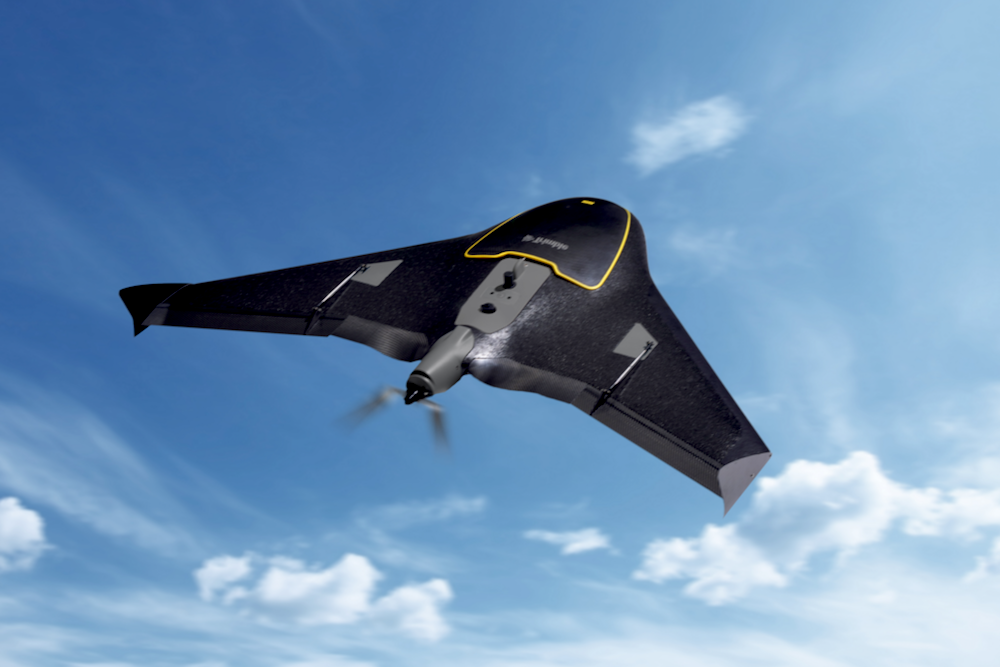
\includegraphics[width=.9\linewidth]{images/fixed-wings-drone.png}
  \caption{Fixed-wing drone}
  \label{fig:uav-fixed-wing}
\end{subfigure}%
\begin{subfigure}{.5\textwidth}
  \centering
  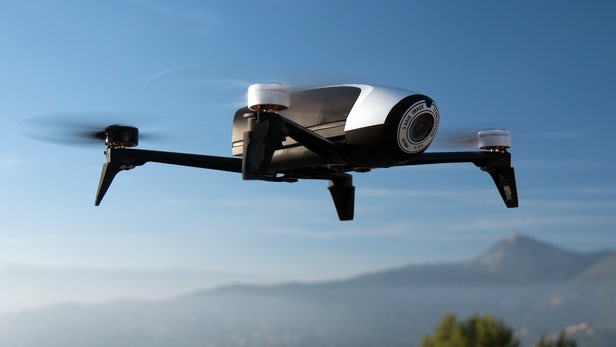
\includegraphics[width=.9\linewidth]{images/quadrotor.jpg}
  \caption{Multi-rotor drone}
  \label{fig:uav-rotor}
\end{subfigure}
\caption{ Two of the most common drone configurations: fixed-wing and the multi-rotor.}
\label{fig:uav-types}
\end{figure}

\glspl{UAV} are classified depending on a wide range of characteristics: size, range, aerial platform, degree of autonomy, engine type and fuel source. All these features are analysed in this section. \\
The first distinction that can be made is based on the type of aerial platform that is used to keep \glspl{UAV} up in the air. Drones available today belongs to one of two main categories: fixed-wing drones and multi-rotor drones. Fixed-wing drones are equipped with fixed, static wings and they use a forward propulsion to move. The way in which they behave is similar to a traditional airplane. Multi-rotor drones, on the other hand, are more similar to helicopters, since they use one or more rotary wings to generate lift. The most common multi-rotor drones use four rotors and are therefore called quadrotors. Depending on the application, one or the other configuration may be more suitable: fixed-wing drones are typically faster than multi-rotors, but they require more space to take off and they can not hover in a fixed position. Multi-rotor drones can overcome these limitations, but are much slower than fixed-wing models.
\glspl{UAV} can be further divided depending on their size and weight. This characteristic reflects the ability of the drone to carry payloads, with bigger drones being able to carry heavy payloads and small drones only able to carry lightweight payloads. Very small \glspl{UAV} have dimensions of 30-50 cm and are usually multi-rotors. Small \glspl{UAV} are slightly larger (up to 1-2 meters along one dimension) and are usually fixed-wing. The same applies to medium and large \glspl{UAV} with the only difference that they can be as big or bigger than a light aircraft. They can carry very heavy payloads (approximately 200 kg) and are generally only used for military applications. 
\glspl{UAV} engines can be powered using many different fuel sources: traditional aircraft fuel (kerosene or gasoline), fuel cells, batteries and solar cells. With the exception of few models, the vast majority of drones are powered either by aircraft fuel or batteries. Drones using aircraft fuel as their power source are able to fly for longer times, but due to the weight of the fuel and the size of the engine, they have bigger dimensions. The most common engines, in order of stability level they can provide, are the four-cycle/two-cycle internal combustion engine, the rotary engine and the gas turbines. Battery-powered drones, equipped with a simple electric motor, are cheap and lightweight, but their flight autonomy is limited to only a few minutes, thus drastically restricting their application in many context.

\subsection{UAV system}

\begin{figure}[h]
    \centering
    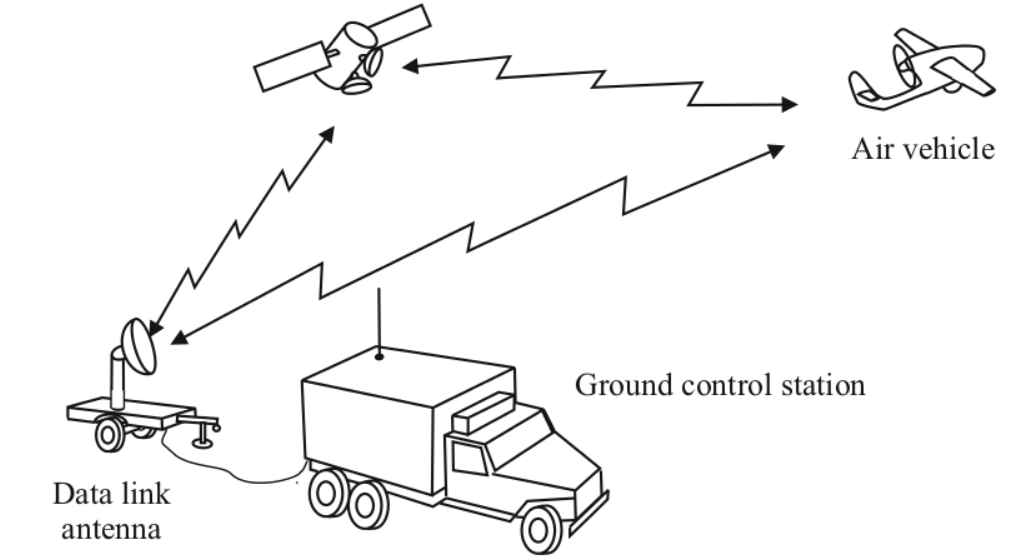
\includegraphics[width=0.9\textwidth]{images/uav-system.png}
    \caption{A general UAV system \ref{undefined}}
    \label{fig:uav-system}
\end{figure}

The operation of one or more \glspl{UAV} requires the deployment of a suitable infrastructure, that is necessary to manage and control all the aspects of the mission. A typical \gls{UAV} system is at least composed by the following elements:

\begin{itemize}
	\item \textbf{Air vehicles:} they are the core part of the system. In order to fly with a high degree of autonomy, air vehicles need to be equipped with some sort of controller that regulate, for example, the altitude and the airspeed. This control is usually achieved by using a feedback or closed-loop controller in conjunction with a set of sensors that typically include an altimeter, a speed meter and some sort of positioning device (a GPS for example). The measurements of the sensors are used by the controller to compute the right actuation to adjust the roll, pitch and/or yaw of the vehicle. Typically the control is limited to one axis (roll) or two axis (roll + pitch) to limit the controller complexity. Almost all \glspl{UAV} are nowadays equipped with a GPS, that can be used to complement the measurements of the other sensors and for accurate path planning;
	
	\item \textbf{Payload:} drones' main mission is to carry a payload. Typical payloads include HD cameras, communication gateways, infrared sensors and thermal sensors. The payload greatly influence the characteristics of the drone that carries it. For example, a heavy payload may require a bigger and more powerful drone;
	
	\item \textbf{\gls{GCS}:} it is usually a vehicle that can transport the drones to the place where they need to operate. The \gls{GCS} is also equipped with all the necessary instruments to process and display the data received from the drones payloads. If the \gls{UAV} system is small, the \gls{GCS} can be reduced to the size of a backpack that can be carried around by the drones operator. A \gls{GCS} can also be located at a fixed position, for example in a building;
	
	\item \textbf{Data link antennas:} antennas are used to establish a two way communication with the air vehicles. The channel is typically split in two sub channels: a low rate channel for transmitting control commands and receiving feedback from the \glspl{UAV} and a high rate channel for receiving sensors data (e.g. the video stream). \gls{LOS} is usually required for the communication to happen;
	
	\item \textbf{\gls{GSE}:} this unit is used to maintain the \glspl{UAV} and may contain spare parts and additional fuel or batteries to extend the \glspl{UAV} on-air time. The \gls{GSE} unit is optional, but its use is generally required, especially in systems with many drones and for missions that require extended operation times.
	
\end{itemize}

%Exclusive prerogative of the military for many years, \glspl{UAV} and drones are now commercially available and their relatively low price makes them appealing for a wide variety of scenarios and applications. The price range can vary between 20\$-300\$ for small battery-powered \gls{RF} drones such as the Parrot Bebop 2, to more than 3000\$ for professional drones with advanced control systems and sensors such as the DJI Spreading Wings S1000. In the consumer market segment, drones are mainly used for taking aerial pictures and videos, while in the commercial segment the range of applications is more diverse: mapping of geographical areas, product delivery and logistic, data collection, crop monitoring and surveillance. Drones are increasingly being used also in civil applications such as crime prevention, weather and meteorology, search and rescue operations, border and maritime patrol and forest fire monitoring. Using \glspl{UAV} provide many advantages compared to ground-based solutions, such as movement in an obstacle-free environment, better overview of the monitored area, presence of \gls{LOS} between the drone and the targets and faster data acquisition over large areas. On the other side, \glspl{UAV} are still limited in terms of flying range, degree of autonomy and flying time. To overcome such issues, \glspl{UAV} swarms are increasingly being considered as a possible solution and many efforts are being directed in the development of suitable communication protocols and swarm mobility models.  